% Figure 2: the clock replacement algorithm, as in ClockBufferManager::alloc_buf.
% Build with:
%   pdflatex clock_flowchart.tex
%   pdftocairo -png -r 200 -singlefile clock_flowchart.pdf clock_flowchart
\documentclass[tikz,border=8pt]{standalone}
\usepackage[T1]{fontenc}
\usepackage{lmodern}
\usetikzlibrary{arrows.meta,positioning,shapes.geometric}

\definecolor{terminal}{HTML}{E3F2FD}
\definecolor{decision}{HTML}{FFF8E1}
\definecolor{fail}{HTML}{FFEBEE}
\definecolor{done}{HTML}{E8F5E9}

\begin{document}
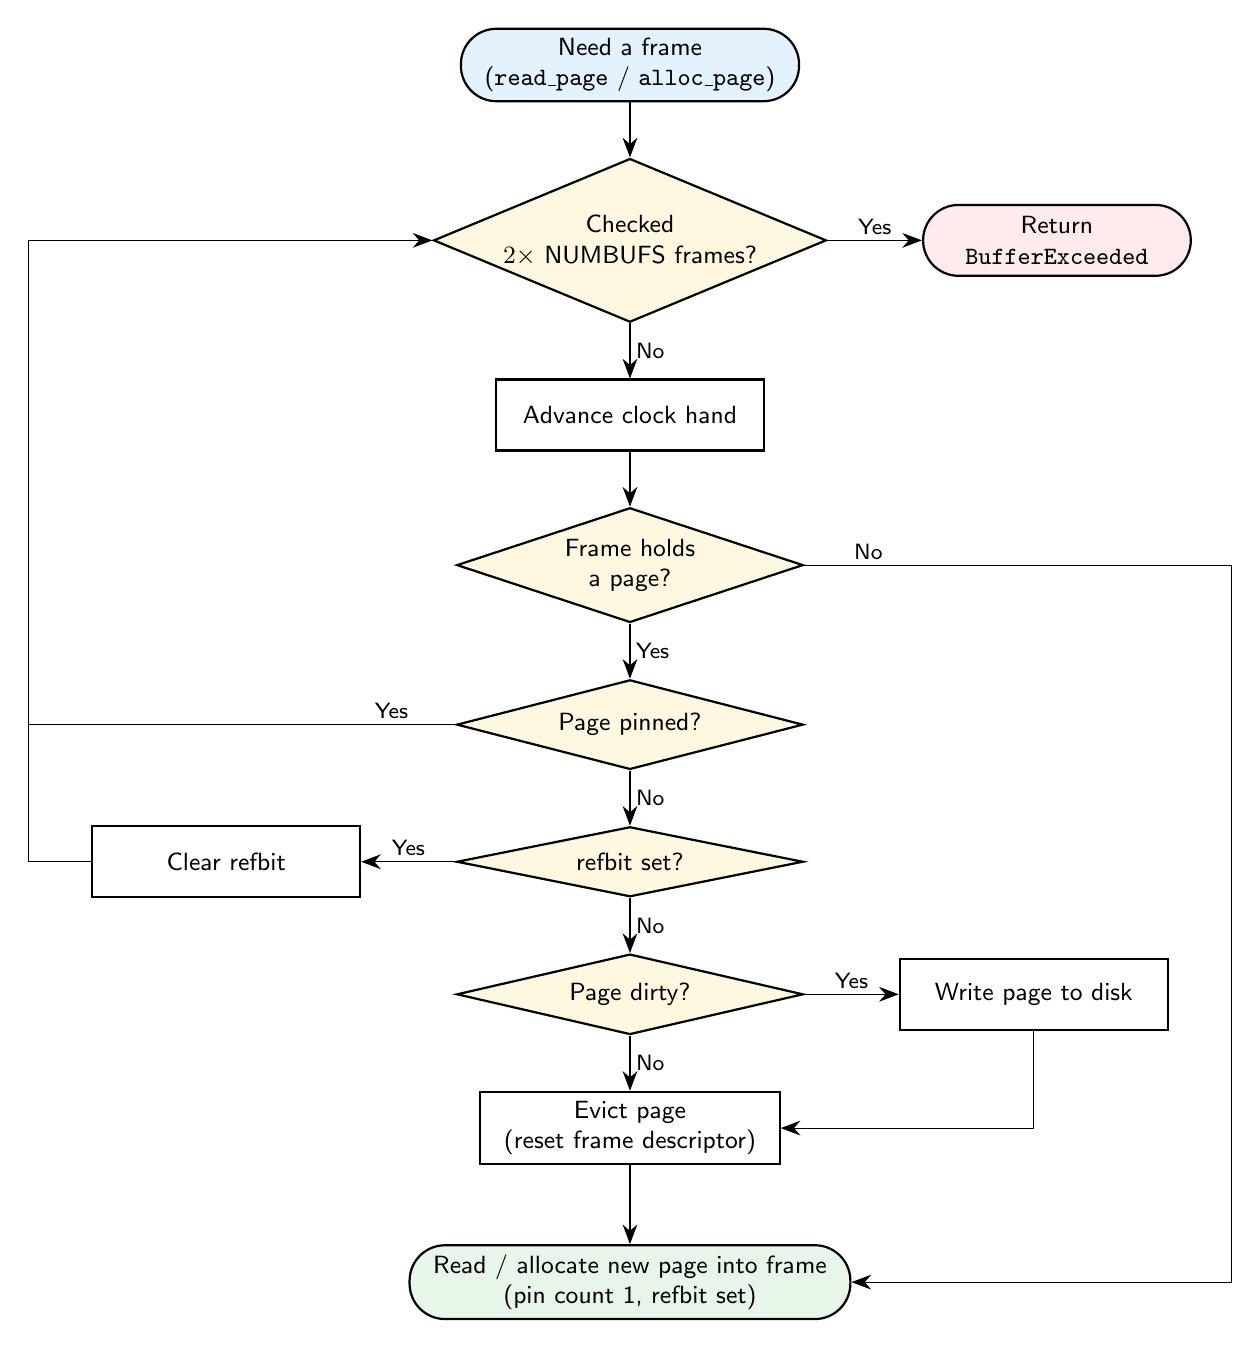
\begin{tikzpicture}[
    font=\sffamily\small,
    node distance=7mm and 12mm,
    >={Stealth[length=2.5mm]},
    every edge/.style={draw, ->},
    proc/.style={draw, thick, rectangle, minimum width=34mm, minimum height=9mm,
                 inner xsep=3mm,
                 align=center, fill=white},
    term/.style={proc, rounded corners=4.5mm, fill=terminal},
    test/.style={draw, thick, diamond, aspect=2.4, inner sep=1pt, align=center,
                 minimum width=44mm,
                 fill=decision},
    lbl/.style={font=\sffamily\footnotesize, inner sep=2pt},
  ]
  % Main column.
  \node[term] (start) {Need a frame\\(\texttt{read\_page} / \texttt{alloc\_page})};
  \node[test, below=of start] (bound) {Checked\\$2 \times$ NUMBUFS frames?};
  \node[proc, below=of bound] (advance) {Advance clock hand};
  \node[test, below=of advance] (valid) {Frame holds\\a page?};
  \node[test, below=of valid] (pinned) {Page pinned?};
  \node[test, below=of pinned] (ref) {refbit set?};
  \node[test, below=of ref] (dirty) {Page dirty?};
  \node[proc, below=of dirty] (clear) {Evict page\\(reset frame descriptor)};
  \node[term, fill=done, below=10mm of clear] (use)
    {Read / allocate new page into frame\\(pin count 1, refbit set)};

  % Side actions.
  \node[term, fill=fail, right=of bound] (exceeded) {Return\\\texttt{BufferExceeded}};
  \node[proc, left=of ref] (clearref) {Clear refbit};
  \node[proc, right=of dirty] (write) {Write page to disk};

  % Straight-through ("No"/"Yes") path down the main column.
  \draw[->] (start) -- (bound);
  \draw[->] (bound) -- node[lbl, right] {No} (advance);
  \draw[->] (advance) -- (valid);
  \draw[->] (valid) -- node[lbl, right] {Yes} (pinned);
  \draw[->] (pinned) -- node[lbl, right] {No} (ref);
  \draw[->] (ref) -- node[lbl, right] {No} (dirty);
  \draw[->] (dirty) -- node[lbl, right] {No} (clear);
  \draw[->] (clear) -- (use);

  % Branches to the right.
  \draw[->] (bound) -- node[lbl, above] {Yes} (exceeded);
  \draw[->] (dirty) -- node[lbl, above] {Yes} (write);
  \draw[->] (write) |- (clear);
  % An empty frame is used right away.
  \coordinate (emptyx) at ([xshift=8mm]write.east);
  \draw[->] (valid.east) -- node[lbl, above, pos=0.15] {No}
    (valid.east -| emptyx) -- (use.east -| emptyx) -- (use.east);

  % Loop back to the bound check; the clock keeps sweeping.
  \coordinate (loopx) at ([xshift=-8mm]clearref.west);
  \draw[->] (ref) -- node[lbl, above] {Yes} (clearref);
  \draw (clearref.west) -- (clearref.west -| loopx);
  \draw (pinned.west) -- node[lbl, above, pos=0.15] {Yes} (pinned.west -| loopx);
  \draw[->] (clearref.west -| loopx) -- (bound.west -| loopx) -- (bound.west);
\end{tikzpicture}
\end{document}
